\documentclass[10pt,twocolumn,letterpaper]{article}


\usepackage{minted}
\usepackage{cvpr}
\usepackage{times}
\usepackage{epsfig}
\usepackage{graphicx}
\usepackage{caption}
\usepackage{subcaption}
\usepackage{dcolumn}
\usepackage{amsmath}
\usepackage{amssymb}
\usepackage{xcolor}
\definecolor{bg}{rgb}{0.95,0.95,0.95}


% Include other packages here, before hyperref.

% If you comment hyperref and then uncomment it, you should delete
% egpaper.aux before re-running latex.  (Or just hit 'q' on the first latex
% run, let it finish, and you should be clear).
\usepackage[breaklinks=true,bookmarks=false]{hyperref}

\cvprfinalcopy % *** Uncomment this line for the final submission

\def\cvprPaperID{****} % *** Enter the CVPR Paper ID here
\def\httilde{\mbox{\tt\raisebox{-.5ex}{\symbol{126}}}}

% Pages are numbered in submission mode, and unnumbered in camera-ready
%\ifcvprfinal\pagestyle{empty}\fi
\setcounter{page}{4321}
\begin{document}

%%%%%%%%% TITLE
\title{Textons and classifiers laboratory report}

\author{José Antonio Valero Medina\\
Universidad Distrital "Francisco José de Caldas"\\
Carrera 7 No. 40B - 53, Bogotá D.C. - República de Colombia\\
{\tt\small jvalero@udistrital.edu.co}
% For a paper whose authors are all at the same institution,
% omit the following lines up until the closing ``}''.
% Additional authors and addresses can be added with ``\and'',
% just like the second author.
% To save space, use either the email address or home page, not both
}

\maketitle
%\thispagestyle{empty}

%%%%%%%%% ABSTRACT
\begin{abstract}
   Here it is reported and discussed a code creation to represent images using textons in order to train and test nearest neighbor and random forest classifiers. Whole process was run on database with a training dataset of 750 images for 25 texture categories and a test dataset of 250 images for the same 25 texture categories. First, the training dataset was filtered using a filter bank made of 32 oriented filters and two center surround ones.  From each filter bank processed image was taken only 1 pixel for each 256 of them in order to be able to manage a possible memory lack in k-means clustering.  Next, 200 textons were produced using the k-means grouping. Then, each image, in both training and test datasets, had its filter bank processed pixels linked to the nearest texton, \ie cluster centroid location. Finally, the texton normalized frequency distribution (histogram) on each image was calculated and used as a descriptor for it in the database. So the training and test datasets was produced and used in the classification stage to train and predict the test image class, \ie texture category, using a nearest neighbor and a random forest classifiers. The classification evaluations showed that the best classifier was the random forest one.
\end{abstract}

%%%%%%%%% BODY TEXT
\section{Introduction}

Here it is reported and discussed a code creation to represent images using textons in order to train and test nearest neighbor and random forest classifiers. Whole process was run on database with a training dataset of 750 images for 25 texture categories and a test dataset of 250 images for the same 25 texture categories.

First, each training dataset image was filtered using a filter bank made of 32 oriented filters and two center surround ones. The procedure followed for it in the included example script, \ie to mosaic the images to form only one,  was not followed here as the filter bank process aborted with a lack of memory error. Instead, each training image was individually filter bank processed.  From each so produced image was taken only 1 of each 256 pixels in order to be able to manage a possible memory lack in k-means clustering. So sampled images, with 30 X 40 pixels, were stacked all together to form an image of 30 x 25 rows and 40 x 30 columns as there were 25 texture categories and each texture category had 30 variations.

Next, 200 textons, \ie k-means clusters each one represented by the respective cluster centroid location, were produced. Then, each image, in both training and test datasets, had its filter bank processed pixels linked to the nearest texton, \ie nearest cluster centroid location, using \textit{assignTextons} provided function. Finally, a texton normalized frequency distribution (histogram) on each image was calculated and used as its descriptor in the database.

After having assigned a descriptor to each database image and produced training and test datasets,  the classification stage was conducted. Two classifiers, a nearest neighbor and a random forest, were trained with the training dataset and used to predict the texture category of each test image in the testing dataset. \textit{chi2} function was implemented as nearness measure for the nearest neighbor classifier and a bag with 50 decision trees was used for the random forest one. The classification evaluation stage was done using a confusion matrix from which the overall accuracy and  texture category accuracy vector measurements were produced. The classification evaluation outcome  showed that the best classifier was the random forest one as this nearly doubled overall accuracy obtained by nearest neighbor.

%-------------------------------------------------------------------------
\section{Data and methods}

\subsection{Functions in \textit{lib} folder}

\textit{fbCreate} creates a filter bank at different scales containing even and odd symmetric filters in several orientations (except center surround filter as the respective creation code line is included but commented out). Each orientation is calculated as a $\pi$ fraction depending on the wanted number of orientation (8 by default) and the scale (a given maxnification scaling rate). An elongation ratio, which should be greater than 1, determines how elongated, along the orientation, the border is. For each orientation (and scale) two filters are built optionally doing for one of them a Hilbert transform in \textit{y} direction but using for both a second \textit{y} derivative. oeFilter function is used to create each filter in the bank. oeFilter produces a Gaussian square odd sized filter with a given orientation. The filter is built seizing the Gaussian separability feature applying \textit{L1-norm} at the end.

\textit{fbRun} applies a filter bank to an image reflecting its boundary border in agreement with the greater filter size found in the filter bank. If a filter size is less than 50 this makes a convolution otherwise this calculates a 2-D inverse fast Fourier transform of the product between 2-D fast Fourier transform on the image and filter. This function returns a cell with a filtered image for each filter in the filter bank organized as the filter bank by orientation and scale.

\textit{computeTextons} produces, based on a k-means grouping, a wanted number of \textit{textons} classes from a filtered image set. Each filtered image corresponds to a dimension of the new feature space with as many dimension as the number of images in the filtered image set. The k-means grouping method is applied on the new feature space for creating as many \textit{textons} as the number of clusters so generated, \ie each cluster is a \textit{texton}. Finally, this function returns an image whose pixel values correspond with the \textit{texton} class, \ie cluster code as generated by k-means, as a \textit{Map} and the cluster centroid locations for each cluster as the descriptor for each \textit{texton} class in the \textit{textons} matrix.

\textit{assignTextons} assigns a texton to a filtered image set based on a \textit{textons} matrix, \ie a matrix whose rows corresponds with a texton and the respective column value set with the cluster centroid location. The filtered image set must have as many filtered images as the second dimension size of \textit{texton} matrix. The filtered image set is put in a feature space whose elements are assigned to the nearest texton, \ie nearest to the respective cluster centroid location taking the squared distance as the nearness measurement. Finally, this function returns an image whose pixel values correspond with the \textit{texton} class (\ie cluster code as generated by k-means) as a \textit{Map}.

\subsection{Database}

The database downloaded from \url{http://157.253.63.7/textures.tar.gz} is made of training and test texture gray scale images. This database provides 25 different categories of texture each one with 30 variations in the training dataset and 10 in the test one. The variations can be in orientation, and scale. The database also includes a dictionary which provides a semantic value for each category.

\subsection{Methods}

The procedure followed in the included example script, \ie to mosaic the images to form only one,  was not followed here as the filter bank and k-means grouping processes aborted with a lack of memory error.  In the following implemented custom matlab functions are discussed.

First activity was to adjust the \textit{fbCreate} algorithm since it had included  center surround filter creation but as comment. The respective line code was \textit{Uncomment} in matlab and the csFilter invoked  was created as that available in \url{https://github.com/jflalonde/colorRealism/blob/master/3rd_party/segmentationBerkeley/lib/matlab/csFilter.m}. It was necessary to do that because some textures were center surround ones.

\textit{DatabaseDescTiTj} function was implemented to produce the texton descriptors of the database. First, each training dataset image was individually filtered using a filter bank made of 32 oriented filters and two center surround ones. Next, from each so produced image was taken only 1 of each 256 pixels in order to be able to manage a possible memory lack in k-means clustering. So sampled images, with 30 X 40 pixels, were stacked all together to form an image of 30 x 25 rows and 40 x 30 columns as there were 25 texture categories and each texture category had 30 variations. Finally, 200 textons, \ie k-means clusters each one represented by the respective cluster centroid location, were produced using \textit{computeTextons} provided function. \textit{DatabaseDescTiTj} is invoked for being executed between two texture categories from the starting one (tIni) and the ending one (tEnd). Both the filter bank processed pixel sampled set and the produced texton set are saved on disk.

\textit{assignDesc} function performs the following process for each image in the dataset. First it runs the filter bank, using \textit{fbRun} provided function, and assign the texton to each pixel, using \textit{assignTextons} provided function. On the so marked image \textit{assignDesc} calculates a texton normalized frequency distribution (histogram) and used it as the image descriptor  and adds the respective vector to the descriptor dataset. The final image descriptors can optionally have a predictor column.

\textit{nearestNeighborClassifier} function first creates a nearest neighbor classifier based on the training dataset provided and then uses it to predict the class of each descriptor in the test dataset provided using chi square distance as a similarity measure. The last column in the provided training dataset will be used as the predictor one. As many columns as there are before the last column in the training dataset are used from the provided testing dataset.

\textit{randomForestClassifier} function first creates and trains a random forest classifier model based on the training dataset provided and then uses it to predict the class of each descriptor in the test dataset provided. The model bags 50 decision trees. As many columns as there are before the last column in the training dataset are used from the provided testing dataset.

\textit{chi2} function implements chi square similarity metric but as required by fitcknn funcion used in nearest neighbor classifier as is shown in the following \textit{matlab} function snip:

\begin{minted}[bgcolor=bg]{matlab}
                 	...
                	
d2 = zeros(size(h2,1),1);
    
for j = 1:size(h2,1)
 d2(j) = ...
   sum(((h1 - h2(j,:)).^2)./(h1 + h2(j,:)));
end
    
                    ...
\end{minted}




Whole applied procedure is included in the \textit{Classifier} matlab script. First, the filter bank is created using the default options to produce 34 filters. After, texton descriptors are created in a sampled way as described before using 200 textons as with them was possible to get a good overall accuracy for the random forest classifier as shown below. Then, the training and test image descriptors were created with a predictor column for both dataset. This predictor is used in the case of the test dataset only during classification evaluation stage for producing the confusions matrices. After having assigned a descriptor to each database image and produced training and test datasets,  the classification stage was conducted. Two classifiers, a nearest neighbor and a random forest, were trained with the training dataset and used to predict the texture category of each test image in the testing dataset. \textit{chi2} function was implemented as nearness measure for the nearest neighbor classifier and a bag with 50 decision trees was used for the random forest one. The classification evaluation stage was done using a confusion matrix (as shown in the following \textit{matlab} function snip) from which the overall accuracy and  texture category accuracy vector measurements were produced. The classification evaluation outcome  showed that the best classifier was the random forest one as this nearly doubled overall accuracy obtained by nearest neighbor.

\begin{minted}[bgcolor=bg]{matlab}
			...
			
%% Evaluate nearest neighbor classification
    % Overall accuracy
confNearNeig = ...
  confusionmat(testData(:,201), ...
  classifNearNeig);
TPNN = sum(diag(confNearNeig));
overallAccuracyNN = ...
  TPNN / sum(sum(confNearNeig));

    % Texture category accuracy
textureCategAccNN = ...
  diag(confNearNeig)./sum(confNearNeig,2);

%% Evaluate random forest classification
    % Overall accuracy
confRanFor = ...
  confusionmat(testData(:,201), ...
  cellfun(@str2num,classifRanFor));
TPRF = sum (diag(confRanFor));
overallAccuracyRF = TPRF/sum(sum (confRanFor));

    % Texture category accuracy
textureCategAccRF = 
  diag(confRanFor)./sum(confRanFor,2);
            
            ...
\end{minted}



\begin{figure*}
    \centering
    \begin{subfigure}[b]{0.2\textwidth}
        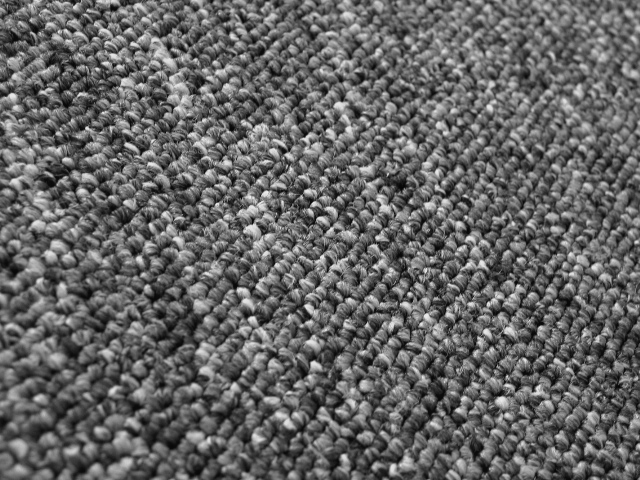
\includegraphics[width=\textwidth]{T18_01.jpg}
    \end{subfigure}
    ~ 
    \begin{subfigure}[b]{0.2\textwidth}
        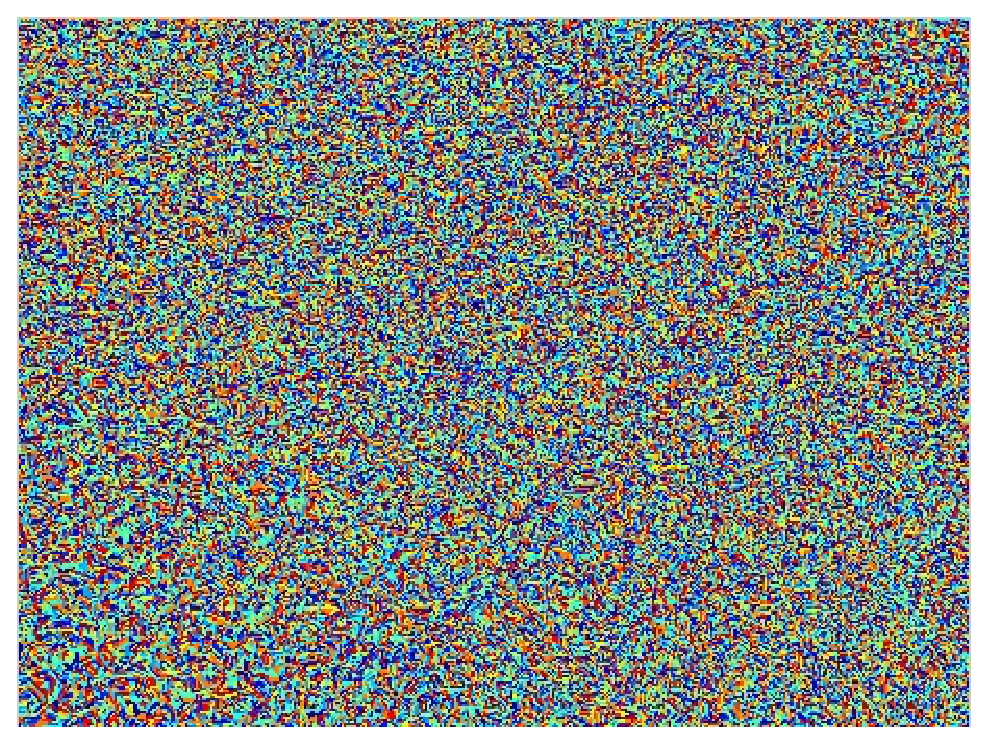
\includegraphics[width=\textwidth]{T18_D01.eps}
    \end{subfigure}
    ~ 
    \begin{subfigure}[b]{0.2\textwidth}
        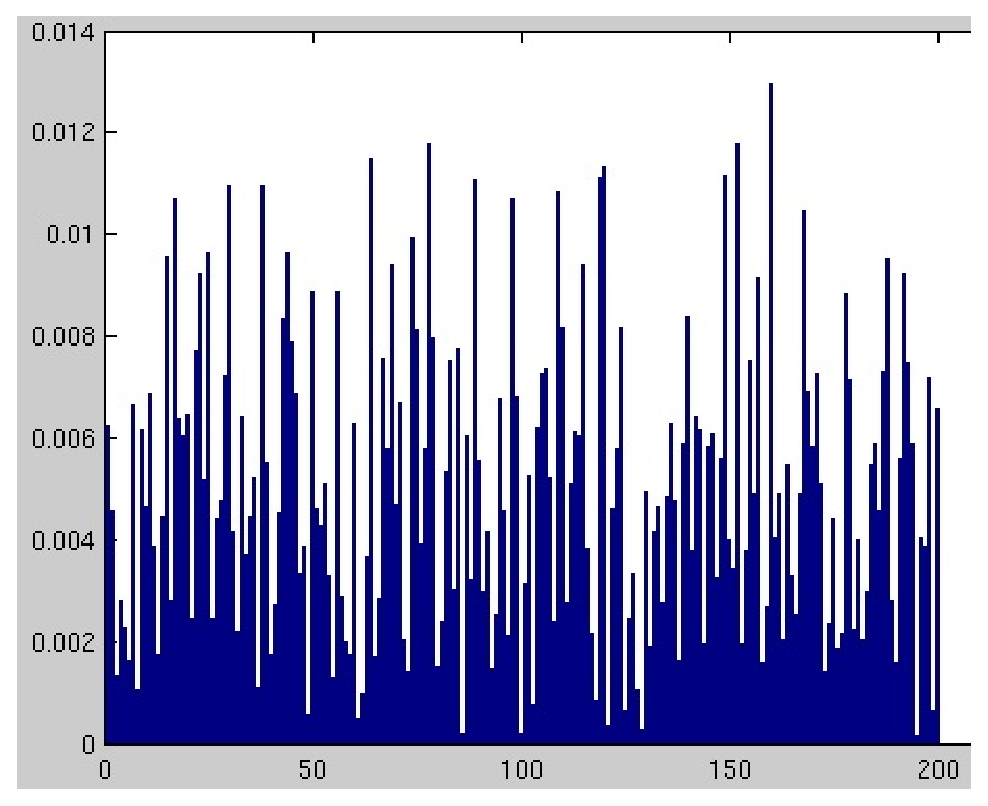
\includegraphics[width=\textwidth]{T18_H01.eps}
    \end{subfigure}
    \\ 
    \begin{subfigure}[b]{0.2\textwidth}
        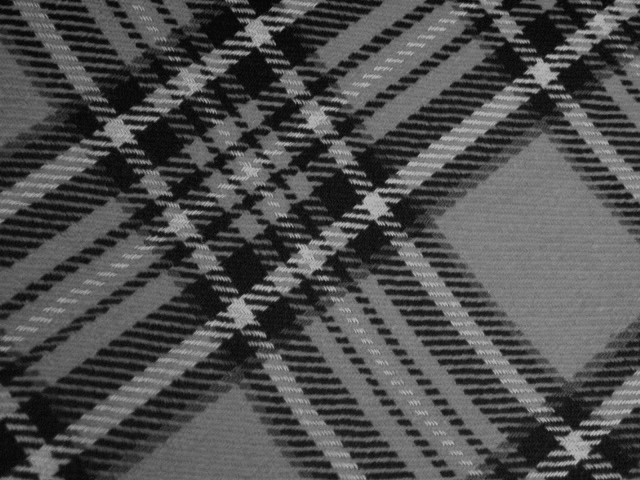
\includegraphics[width=\textwidth]{T25_01.jpg}
    \end{subfigure}
    ~ 
    \begin{subfigure}[b]{0.2\textwidth}
        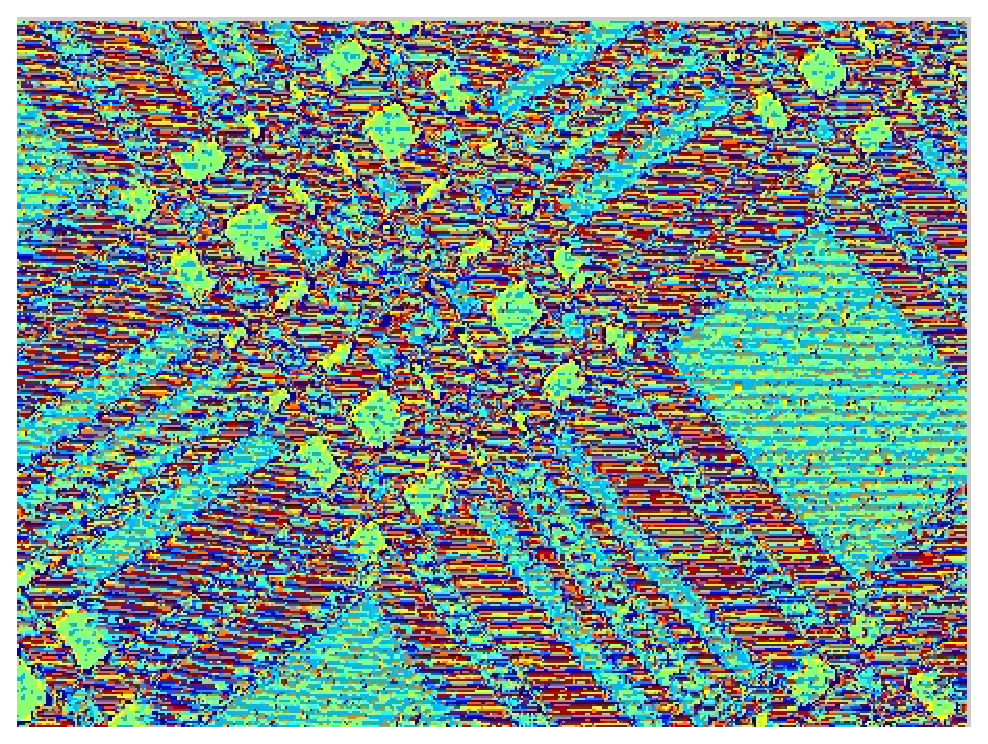
\includegraphics[width=\textwidth]{T25_D01.eps}
    \end{subfigure}
    ~ 
    \begin{subfigure}[b]{0.2\textwidth}
        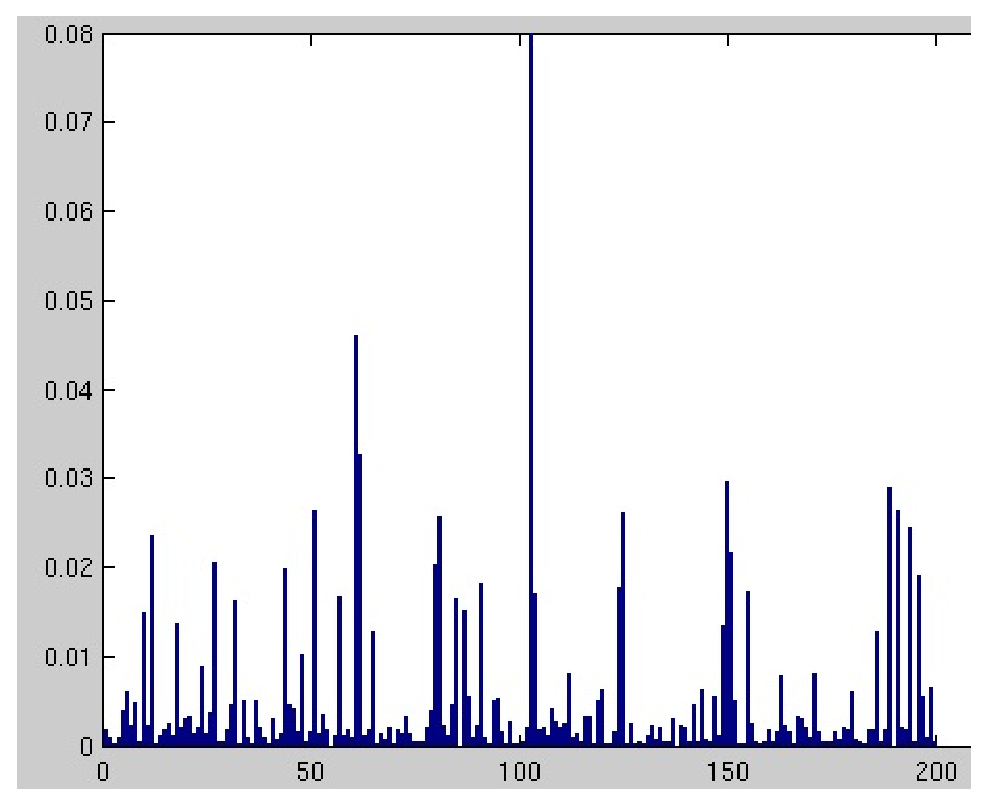
\includegraphics[width=\textwidth]{T25_H01.eps}
    \end{subfigure}
    \\ 
    \begin{subfigure}[b]{0.2\textwidth}
        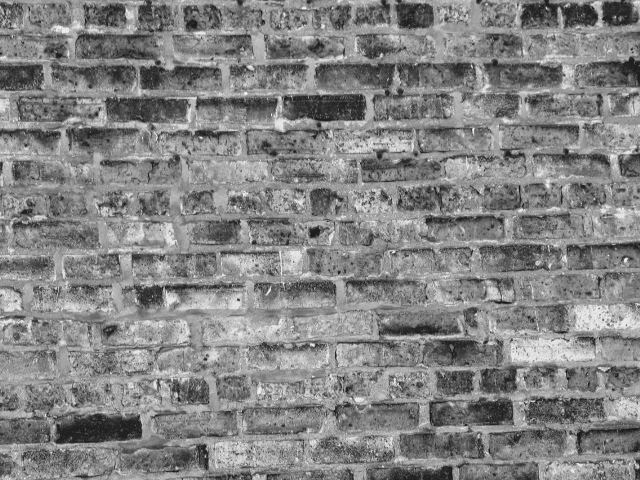
\includegraphics[width=\textwidth]{T14_01.jpg}
    \end{subfigure}
    ~ 
    \begin{subfigure}[b]{0.2\textwidth}
        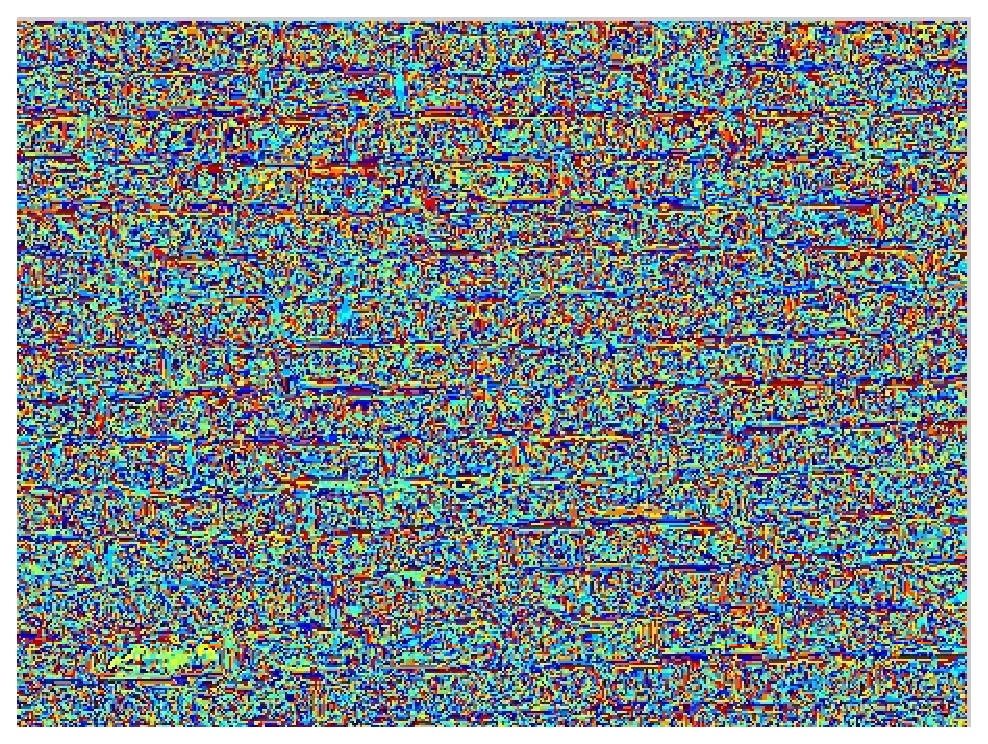
\includegraphics[width=\textwidth]{T14_D01.eps}
    \end{subfigure}
    ~ 
    \begin{subfigure}[b]{0.2\textwidth}
        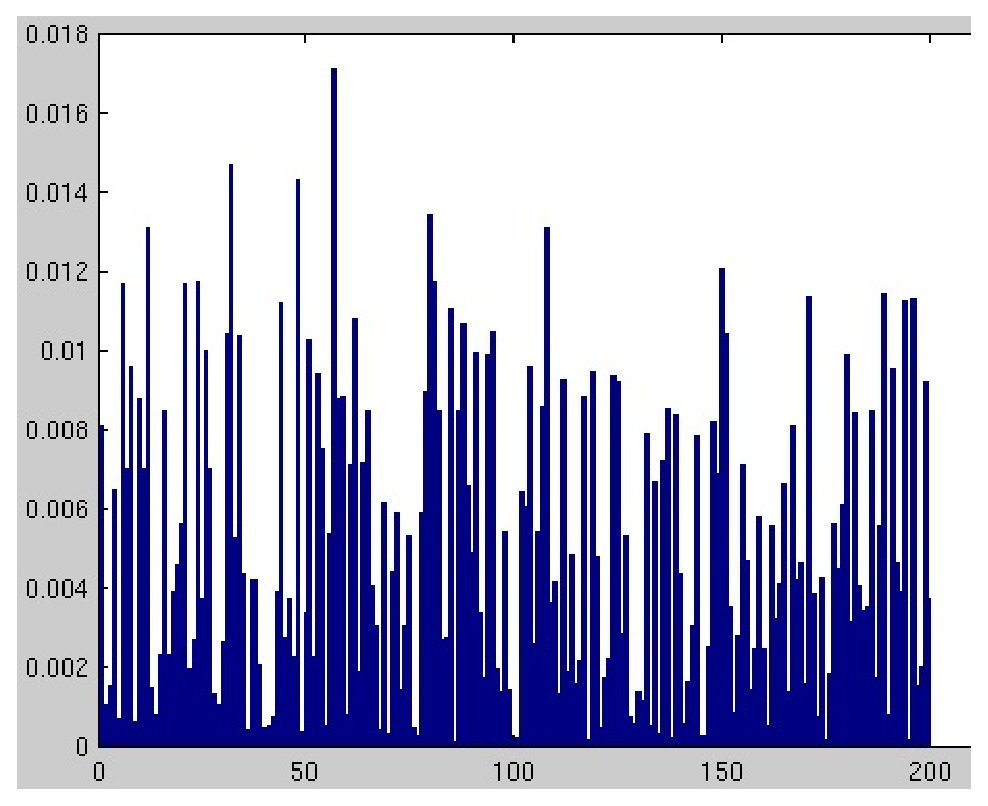
\includegraphics[width=\textwidth]{T14_H01.eps}
    \end{subfigure}
   \caption{Texture categories for carpet (top), plaid (middle) and brick(bottom). Each original texture image (left) is shown with their texton assignment (center) and histogram descriptor (right).}
   \label{fig:imagedesc}
\end{figure*}

\begin{table}
\begin{center}
\begin{tabular}{|c|c|c|}
\hline
Ground truth code& Near.Neig. & Rand.For. \\
\hline\hline
     1  &   1  &   1\\
     2  &   2  &   2\\
     3  &   3  &   3\\
     4  &  12  &   4\\
     5  &   3  &   5\\
     6  &   3  &   6\\
     7  &  22  &  22\\
     8  &   8  &   8\\
     9  &   9  &   9\\
    10  &   9  &  15\\
    11  &  11  &  11\\
    12  &   8  &  12\\
    13  &  13  &  13\\
    14  &   8  &  14\\
    15  &  15  &  15\\
    16  &  16  &  16\\
    17  &   1  &  19\\
    18  &  18  &  18\\
    19  &  19  &  19\\
    20  &  20  &  20\\
    21  &  20  &  10\\
    22  &  12  &  22\\
    23  &  25  &  23\\
    24  &  14  &  24\\
    25  &  25  &  25\\
\hline
\end{tabular}
\caption{Sampled predictions outcomes by each Classifier compared to the ground truth.}
\label{tab:classout}
\end{center}
\end{table}

\begin{table*}
%\begin{center}
\begin{subtable}{.5\textwidth}
%\begin{center}
\begin{tabular}{|c|c|c|c|c|c|c|c|c|c|c|c|c|c|c|c|c|c|c|c|c|c|c|c|c|}
\hline
%& T01&T02&T03&T04&T04&T04&T04&T04&T04&T04&T04&T04&T04&T04&T04&T04&T04&T04&T04&T04&T04&T04&T04&T04&T04\\
%\hline\hline
9 & 0 & 0 & 0 & 0 & 0 & 0 & 1 & 0 & 0 & 0 & 0 & 0 & 0 & 0 & 0 & 0 & 0 & 0 & 0 & 0 & 0 & 0 & 0 & 0 \\
0 & 4 & 0 & 0 & 0 & 0 & 0 & 3 & 0 & 2 & 0 & 0 & 0 & 0 & 0 & 0 & 0 & 0 & 1 & 0 & 0 & 0 & 0 & 0 & 0\\
0 & 0 & 9 & 0 & 0 & 0 & 0 & 0 & 0 & 0 & 1 & 0 & 0 & 0 & 0 & 0 & 0 & 0 & 0 & 0 & 0 & 0 & 0 & 0 & 0\\
0 & 0 & 2 & 0 & 0 & 0 & 0 & 0 & 5 & 1 & 0 & 1 & 0 & 0 & 1 & 0 & 0 & 0 & 0 & 0 & 0 & 0 & 0 & 0 & 0\\
0 & 0 & 10 & 0 & 0 & 0 & 0 & 0 & 0 & 0 & 0 & 0 & 0 & 0 & 0 & 0 & 0 & 0 & 0 & 0 & 0 & 0 & 0 & 0 & 0\\
0 & 0 & 5 & 0 & 0 & 0 & 0 & 0 & 3 & 0 & 0 & 1 & 1 & 0 & 0 & 0 & 0 & 0 & 0 & 0 & 0 & 0 & 0 & 0 & 0\\
1 & 0 & 2 & 0 & 0 & 0 & 0 & 0 & 0 & 0 & 0 & 0 & 0 & 0 & 0 & 0 & 0 & 0 & 0 & 0 & 0 & 6 & 0 & 0 & 1\\
0 & 0 & 0 & 0 & 0 & 0 & 0 & 8 & 0 & 2 & 0 & 0 & 0 & 0 & 0 & 0 & 0 & 0 & 0 & 0 & 0 & 0 & 0 & 0 & 0\\
0 & 0 & 0 & 0 & 0 & 0 & 0 & 0 & 8 & 1 & 0 & 0 & 0 & 0 & 1 & 0 & 0 & 0 & 0 & 0 & 0 & 0 & 0 & 0 & 0\\
0 & 0 & 0 & 0 & 0 & 0 & 0 & 0 & 3 & 4 & 0 & 2 & 0 & 0 & 0 & 0 & 0 & 0 & 0 & 0 & 0 & 1 & 0 & 0 & 0\\
0 & 0 & 0 & 0 & 0 & 0 & 0 & 0 & 1 & 0 & 8 & 1 & 0 & 0 & 0 & 0 & 0 & 0 & 0 & 0 & 0 & 0 & 0 & 0 & 0\\
0 & 0 & 0 & 0 & 0 & 0 & 0 & 1 & 0 & 0 & 0 & 8 & 0 & 1 & 0 & 0 & 0 & 0 & 0 & 0 & 0 & 0 & 0 & 0 & 0\\
0 & 1 & 2 & 0 & 0 & 0 & 0 & 0 & 5 & 0 & 0 & 1 & 1 & 0 & 0 & 0 & 0 & 0 & 0 & 0 & 0 & 0 & 0 & 0 & 0\\
2 & 0 & 0 & 0 & 0 & 0 & 0 & 1 & 0 & 0 & 0 & 2 & 0 & 5 & 0 & 0 & 0 & 0 & 0 & 0 & 0 & 0 & 0 & 0 & 0\\
0 & 0 & 0 & 0 & 0 & 0 & 0 & 0 & 1 & 0 & 0 & 1 & 0 & 0 & 7 & 0 & 0 & 0 & 0 & 0 & 0 & 1 & 0 & 0 & 0\\
0 & 0 & 0 & 0 & 0 & 0 & 0 & 0 & 0 & 0 & 0 & 0 & 0 & 0 & 0 & 10 & 0 & 0 & 0 & 0 & 0 & 0 & 0 & 0 & 0\\
3 & 1 & 0 & 0 & 0 & 0 & 0 & 2 & 0 & 1 & 0 & 0 & 0 & 2 & 0 & 0 & 0 & 0 & 1 & 0 & 0 & 0 & 0 & 0 & 0\\
0 & 0 & 0 & 0 & 0 & 0 & 0 & 0 & 0 & 0 & 0 & 0 & 0 & 0 & 0 & 0 & 0 & 9 & 1 & 0 & 0 & 0 & 0 & 0 & 0\\
0 & 3 & 0 & 0 & 0 & 0 & 0 & 3 & 0 & 0 & 0 & 0 & 0 & 0 & 0 & 0 & 0 & 0 & 4 & 0 & 0 & 0 & 0 & 0 & 0\\
0 & 0 & 0 & 0 & 0 & 0 & 0 & 0 & 0 & 2 & 0 & 0 & 0 & 0 & 0 & 0 & 0 & 0 & 1 & 7 & 0 & 0 & 0 & 0 & 0\\
0 & 0 & 0 & 0 & 0 & 0 & 0 & 0 & 8 & 0 & 0 & 0 & 0 & 0 & 0 & 0 & 0 & 0 & 0 & 2 & 0 & 0 & 0 & 0 & 0\\
0 & 0 & 0 & 0 & 0 & 0 & 0 & 0 & 1 & 1 & 0 & 1 & 0 & 0 & 0 & 0 & 0 & 0 & 0 & 0 & 0 & 7 & 0 & 0 & 0\\
5 & 0 & 0 & 0 & 0 & 0 & 0 & 0 & 1 & 0 & 0 & 0 & 1 & 0 & 0 & 0 & 0 & 0 & 1 & 0 & 0 & 1 & 0 & 0 & 1\\
2 & 0 & 0 & 0 & 0 & 0 & 0 & 0 & 0 & 0 & 0 & 0 & 0 & 4 & 0 & 0 & 1 & 0 & 0 & 0 & 0 & 0 & 0 & 3 & 0\\
2 & 0 & 0 & 0 & 0 & 0 & 0 & 0 & 1 & 0 & 1 & 0 & 0 & 0 & 0 & 0 & 0 & 0 & 0 & 0 & 0 & 0 & 0 & 0 & 6\\
\hline\\
\end{tabular}
%\end{center}
\end{subtable}
\caption{Nearest neighbor classification confusion matrix. Rows are the ground truth and columns the prediction.}
\label{tab:confNN}
%\end{center}
\end{table*}


\section{Results}
 
The outcome of applying the filter bank on each training image can be seen on the  shown in Figure~\ref{fig:imagedesc} which shows  an example. On the figure, beside the original texture image, the assigned texton image and its histogram descriptor are also shown. For every category the filer bank allowed a good discrimination in agreement with the specific texture but the more homogeneous is the texture pattern, the Textones best fit as less orientations there are, and better discrimination is obtained. In the case of plaid texture the final histogram descriptor allows to discriminate the most at its maximum values are more far between them. Now the important thing is that the more different the histograms distributions are, better differentiated will be the respective texture images and it will be easier for a classifier to learn that differences.

A classification outcome sample of 25 test texture images is shown in Table~\ref{tab:classout}. The better random forest classifier overall accuracy (last column) is evident in respect of nearest neighbor.  Table~\ref{tab:confNN} shows the confusion matrix for the nearest neighbor classification in which any of  wood1, wood2, wood3, water,glass2, wallpaper and knit (columns 4,5,6,7,17,21 and 23 respectively) texture images could be classified. This fact can be seen in the accuracy of texture category for both classifiers shown in Table~\ref{tab:texcatacc}. The overall accuracy for the nearest neighbor classification was 0.468 while for the random forest classification was 0.84.

\begin{table}
\begin{center}
\begin{tabular}{|c|c|c|}
\hline
Ground truth code & Near.Neig. & Rand.For. \\
\hline\hline
    1 & 0.9 & 1.0\\
    2 & 0.4 & 0.5\\
    3 & 0.9 & 0.9\\
    4 &   0 & 1.0\\
    5 &   0 & 1.0\\
    6 &   0 & 0.9\\
    7 &   0 & 0.7\\
    8 & 0.8 & 0.8\\
    9 & 0.8 & 0.9\\
   10 & 0.4 & 0.8\\
   11 & 0.8 & 1.0\\
   12 & 0.8 & 0.8\\
   13 & 0.1 & 1.0\\
   14 & 0.5 & 0.7\\
   15 & 0.7 & 1.0\\
   16 & 1.0 & 0.9\\
   17 &   0 & 0.8\\
   18 & 0.9 & 1.0\\
   19 & 0.4 & 0.5\\
   20 & 0.7 & 0.8\\
   21 &   0 & 0.8\\
   22 & 0.7 & 0.7\\
   23 &   0 & 0.8\\
   24 & 0.3 & 1.0\\
   25 & 0.6 & 0.7\\
\hline
\end{tabular}
\caption{Accuracy by texture catecory}
\label{tab:texcatacc}
\end{center}
\end{table}

\section{Discussion}
After evaluating the classification outcomes it is clear that the random forest classifier works best nearly almost doubling the nearest neighbor classification overall accuracy. The training time for the nearest neighbor classifier was virtually zero since only had to create the classifier with the training dataset and the training time for the random forest classifier was of some few seconds. It took a really short time to apply both kinds of classifiers. The most delayed stage is the texture image descriptor production as it is k-means dependent.

Table~\ref{tab:texcatacc} shows that for the nearest neighbor classifier wood1, wood2, wood3, water,glass2, wallpaper and knit (codes 4,5,6,7,17,21 and 23 respectively) texture categories cause the most confusion as were not possible to classify any of that test texture images. For the random forest classifier carpet2 texture category cause the  most confusion.

In order to avoid a lack of memory condition during the k-means clustering was necessary to sample each image until taking in account 1 of each 16 rows and 1 of each 16 rows that means that for each sampled pixel 256 were no considered in the processing losing too much information for the image descriptor production stage.

The texture image database provides a very small number of texture categories, so this number should be incremented in order to be able to evaluate more general algorithms.

The filter bank stage was conducted using the default values, it is possible to make a better choice for a specific filters trying to change and test other parameters, $\eg$ the elongation factor on \textit{y} axis or the scale magnification factor.

\section{Improvements}
It is necessary to research in an alternative grouping method in order to be less vulnerable to lack of memory. Matlab could not be as suitable for this specific topic as it is needed in describing a database based on the texton histogram.


%-------------------------------------------------------------------------


%{\small
%\bibliographystyle{ieee}
%\bibliography{vision}
%}

\end{document}
